\section{Introduction}

\subsection{The Intel 8086}
    The birth of x86 architecture - the very same architecture that the vast majority of desktop computers still use today (or at least some 64-bit variant thereof) - took place just over forty years ago with the release of Intel's revolutionary 8086 16-bit microprocessor.

    While obviously the 8086 pales in comparison to modern processors with a clock-speed of 5 to 10 MHz and the ability to address a megabyte of segmented memory the 8086 was, for its time, more than capable in regards to raw processing power. This power however is not the source of the 8086's acclaim. Rather, the reason the Intel 8086 remains relevant today is because of its unique instruction set and the legacy it created as a result.

    Using real addressing mode, any code written for the original 8086 should (at least theoretically) be able to run on any modern x86 processor (assuming all the required interrupts and hardware are available). Importantly, all innovations in processing technology today rely on the 8086 as a backbone.

\subsection{Why build an emulator?}
    For a long while I have found the prospect of implementing my own emulator intriguing. Even before I began programming, I frequently experimented with running virtual machines and emulators for all manner of different hardware. I particularly enjoyed modifying values within memory of a Nintendo Entertainment System (NES) emulator to observe what effects it would have on the running game.

    While the NES itself is a something of a black box, with an emulator it is possible to see the precise state of the Central Processing Unit (CPU) as it runs, change exactly how it runs and even see the disassembled code running on it in real time. In Figure \ref{figure:fceux} for example, I was able to change the colour scheme in the Legend of Zelda as well as give Link infinite health and access to the best weapons in the game simply by changing a few values in memory.

    \begin{figure}[h]
        \centering
        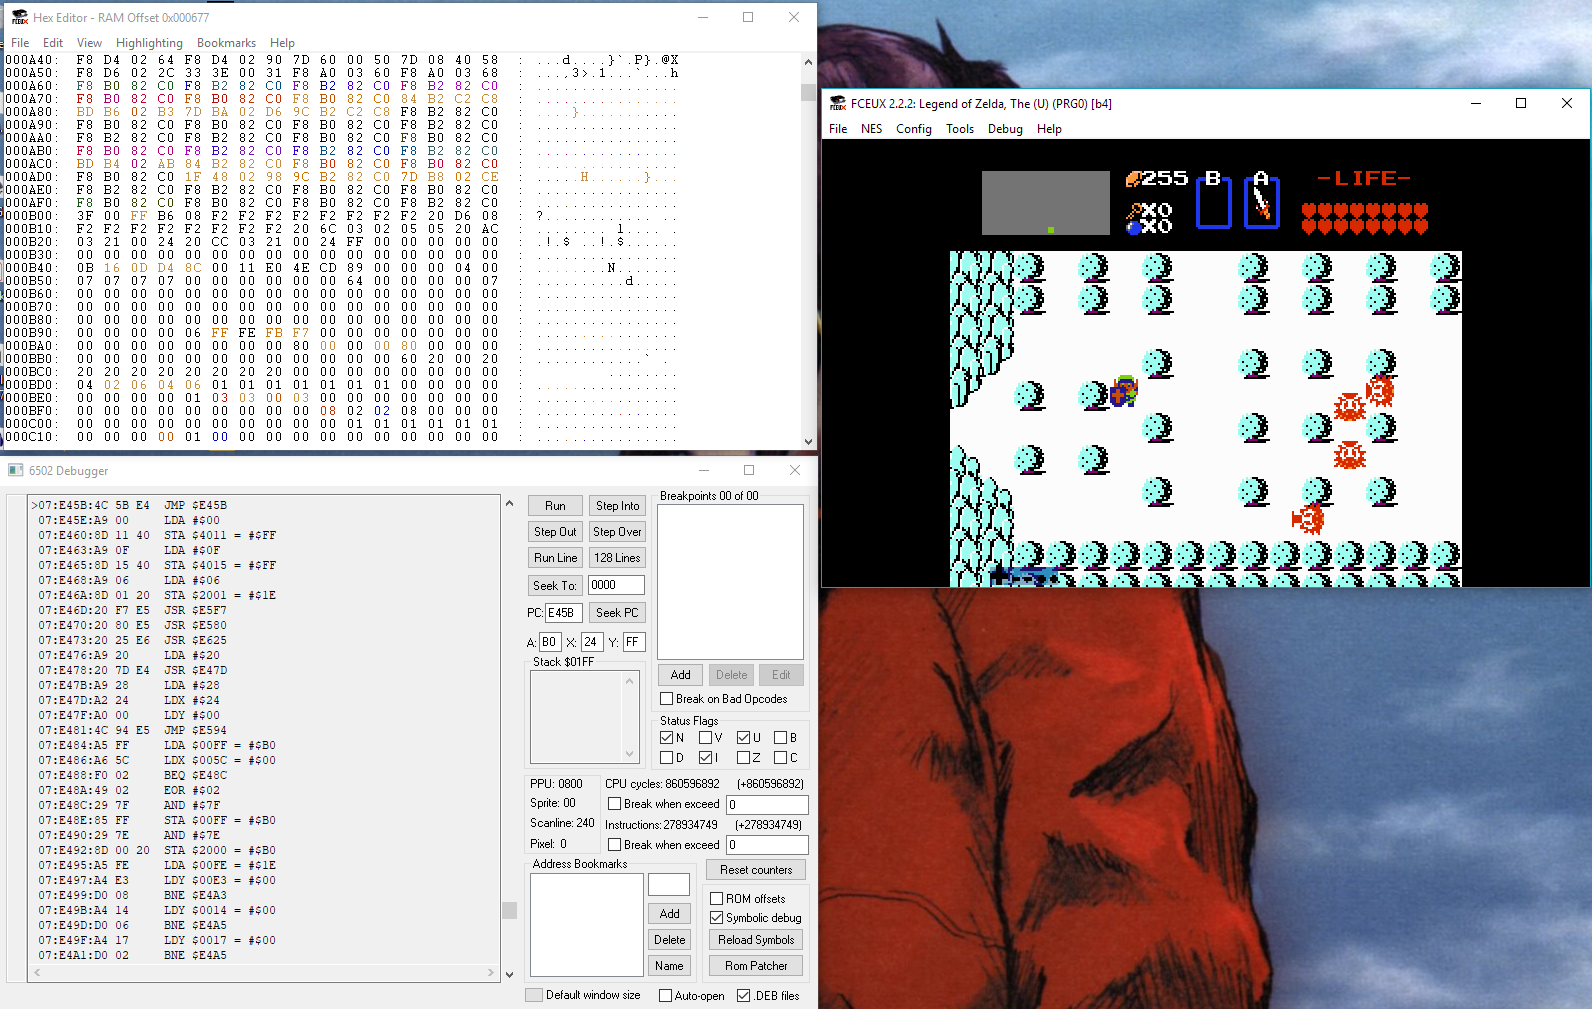
\includegraphics[scale=0.8]{fceux}
        \caption{The Legend of Zelda running in FCEUX with memory modifications.}
        \label{figure:fceux}
    \end{figure}

    In view of this, the key elements for my own emulator are:
    \begin{enumerate}
        \item the ability for the user to view exactly what the CPU is doing at any one time, and
        \item modify its behaviour whilst it is operating.
    \end{enumerate}

    It is not the intention of this project to create a particually fast or complex implementation of the Intel 8086. It is to allow the user to understand what is happening 'under the hood'.

\subsection{Why emulate the Intel 8086?}
    There are a number of reasons as to why I chose to replicate the 8086 specifically. These are summarised as follows:
    \begin{enumerate}
        \item The 8086 had a complexity level high enough to be challenging while not being entirely unapproachable.
        \item Being so well known and having existed for quite some time, there should be a wealth of documentation available for the 8086 online and in books.
        \item Even if the required documentation cannot be found, using disassemblers, hex editing tools and existing emulators, it should be feasible to reverse engineer certain components regardless should there be a need to do so.
    \end{enumerate}

    As mentioned previously, all current x86 processors maintain backwards compatibility with the Intel 8086. This means that, should I wish to implement a more advanced x86 processor in the future, it should be possible to reuse some of the code from this project.

    This was another key point that drew me to the 8086 as, assuming this project is successful, I plan to implement the 32-bit Intel 80386 sometime in the future.